\begin{withoutheadline}
  \begin{frame}{From physics to the mathematical model}
    
  \vspace{-0.6cm}
  \begin{overprint}
    \onslide<1>
    \begin{columns}
      \begin{column}{0.45\textwidth}
        \begin{block}{Solid dynamics problems}
          \begin{itemize}
          \item[] \textbf{Impact; Crash-proof design}
          \item[] High-speed forming
          %\item[] Earthquake reliability of structures 
          \end{itemize}
        \end{block}
      \end{column}
      
      \begin{column}{0.55\textwidth}
      \end{column}
    \end{columns}
    
    \begin{figure}[ht]
      \centering
      \subcaptionbox{Bird strike on aircrafts}{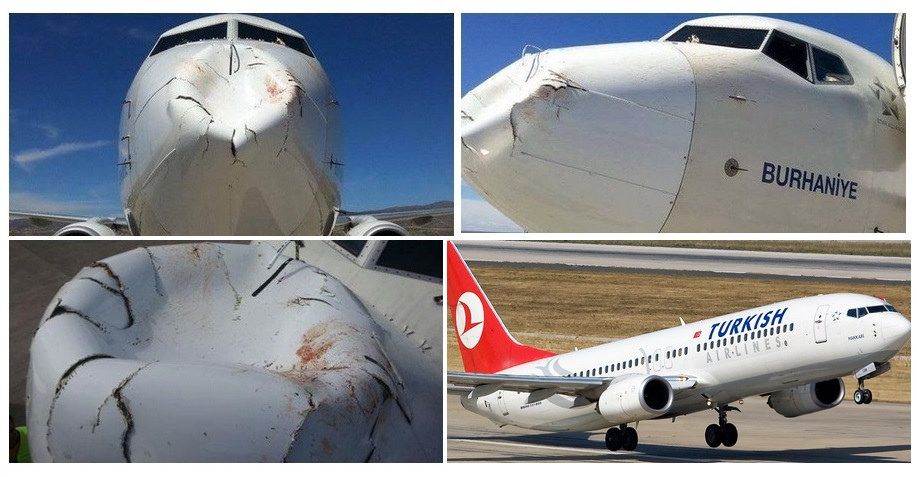
\includegraphics[height=0.3\paperheight]{section1/pictures/birdstrike.jpg}}
      \subcaptionbox{Glasgow Museum of Transport}{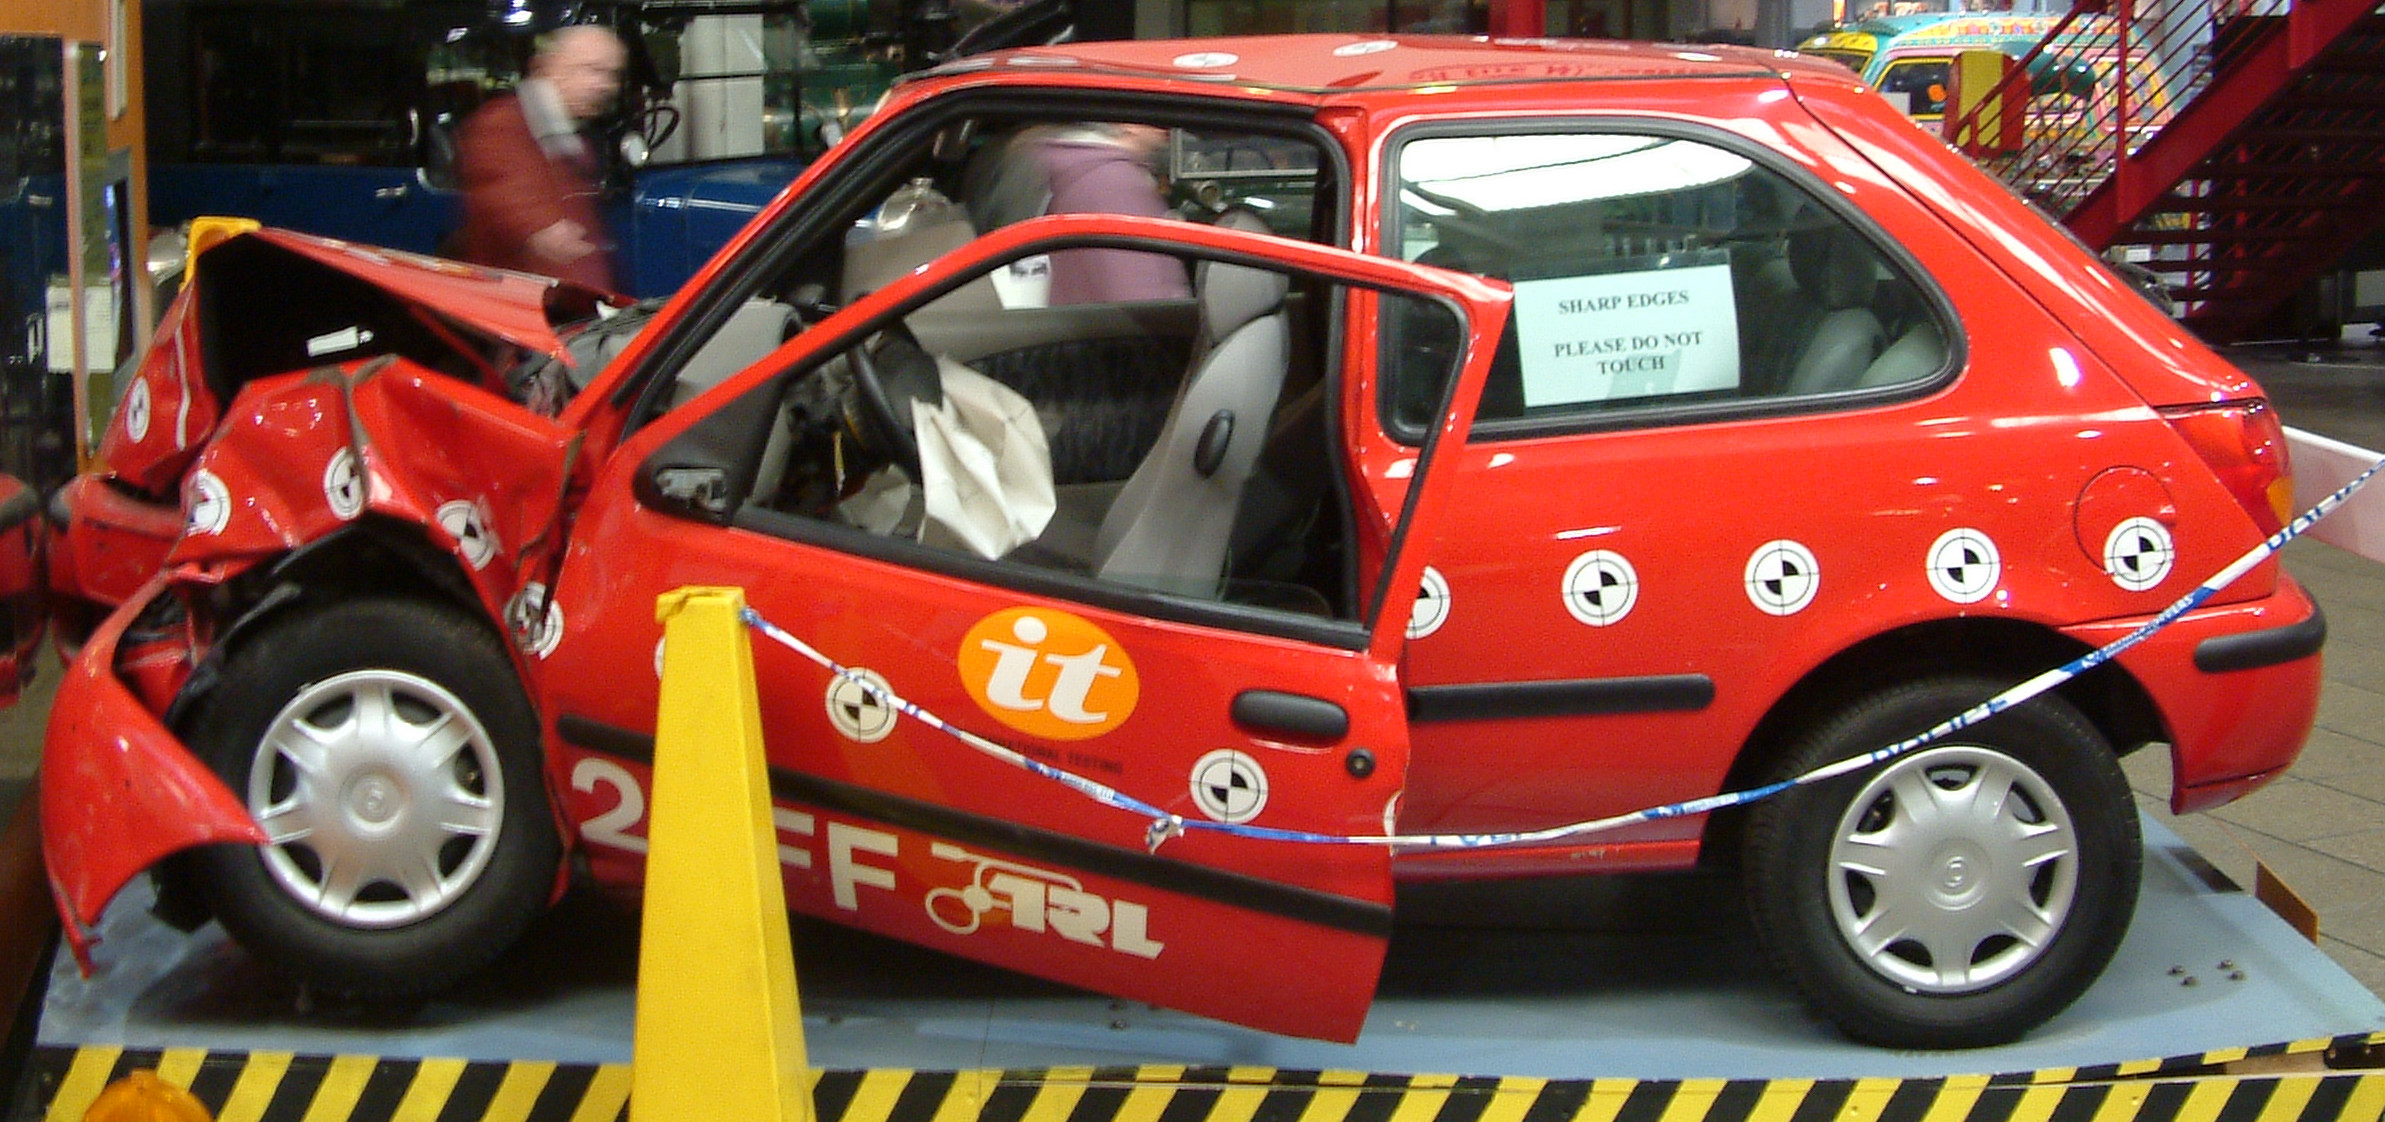
\includegraphics[height=0.3\paperheight]{section1/pictures/crash2.jpg}}
    \end{figure}
    
    \onslide<2>
    \begin{columns}
      \begin{column}{0.45\textwidth}
        \begin{block}{Solid dynamics problems}
          \begin{itemize}
          \item[] Impact; Crash-proof design
          \item[] \textbf{High-speed forming}
          %\item[] Earthquake reliability of structures 
          \end{itemize}
        \end{block}
      \end{column}
      
      \begin{column}{0.55\textwidth}
      \end{column}
    \end{columns}
    \centering
      \movie[height = 0.45\paperheight,width=0.33\linewidth,loop,poster,autostart]{}{%
      section1/animation/output3.mp4}\\
    \scriptsize Electromagnetic forming \cite{Guillaume}
    \footnoteCite{Guillaume}
    
    % \onslide<3>
    % \begin{columns}
    %   \begin{column}{0.45\textwidth}
    %     \begin{block}{Solid dynamics problems}
    %       \begin{itemize}
    %       \item[] Impact; Crash-proof design
    %       \item[] High-speed forming
    %       \item[] \textbf{Earthquake reliability of structures}
    %       \end{itemize}
    %     \end{block}
    %   \end{column}
      
    %   \begin{column}{0.55\textwidth}
    %   \end{column}
    % \end{columns}

    % \centering
    % 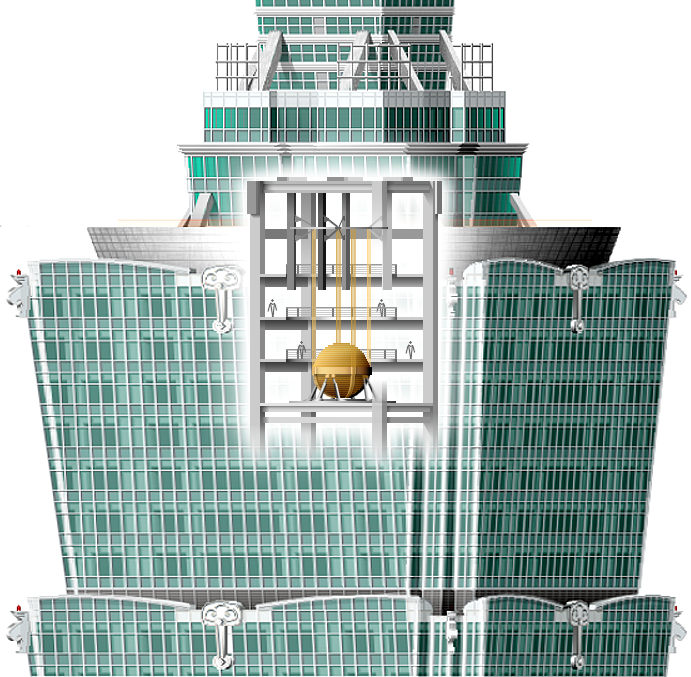
\includegraphics[scale=0.15]{section1/pictures/TaipeiTower.png} \quad
    % 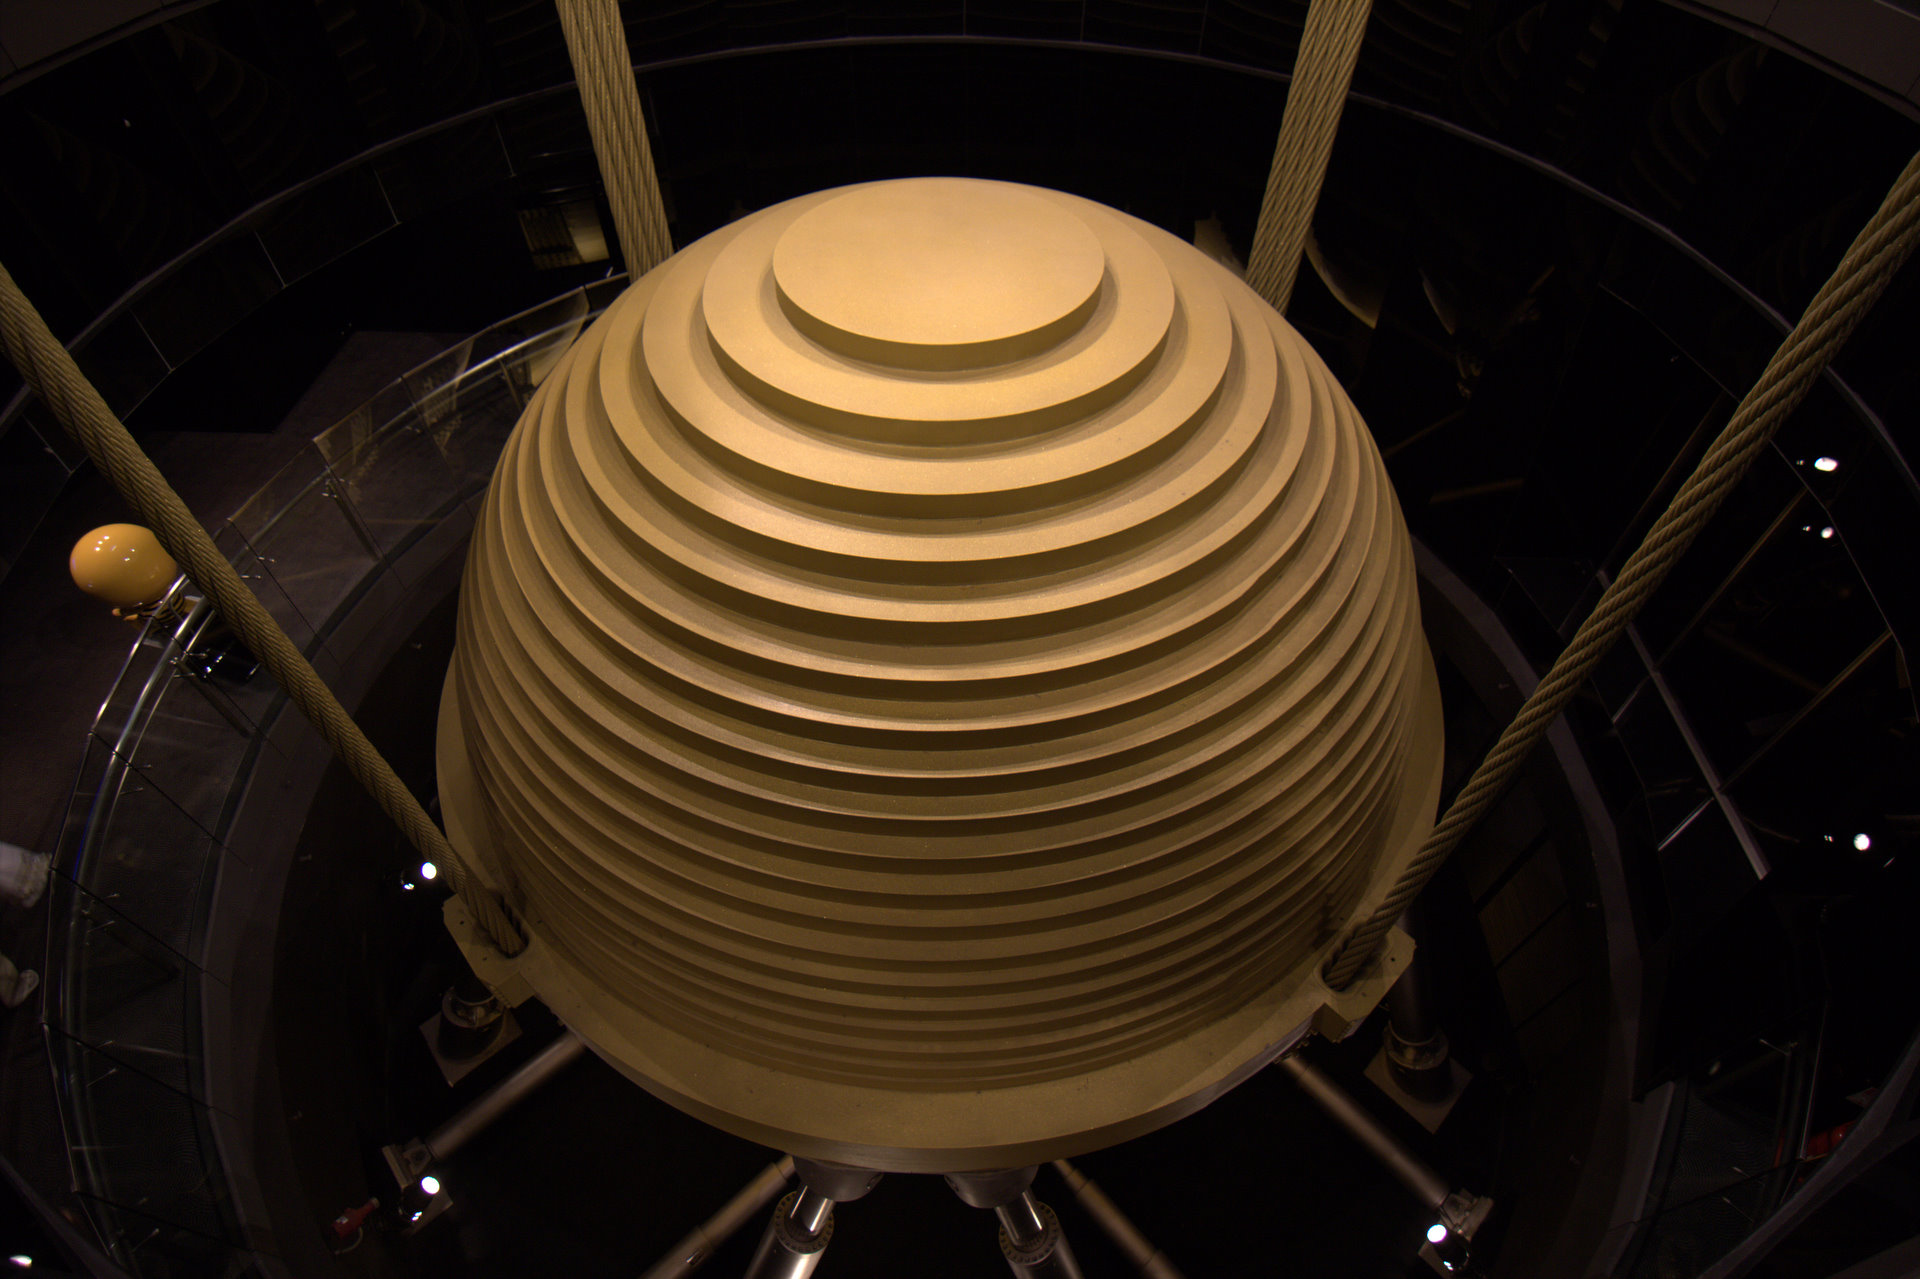
\includegraphics[scale=0.08]{section1/pictures/MassDamper.jpg}\\
    % \scriptsize Taipei 101 mass damper

    \onslide<3>
    \begin{columns}
      \begin{column}{0.45\textwidth}
        \begin{block}{Solid dynamics problems}
          \begin{itemize}
          \item[] Impact; Crash-proof design
          \item[] High-speed forming
          %\item[] Earthquake reliability of structures 
          \end{itemize}
        \end{block}
      \end{column}
      
      
      \begin{column}{0.55\textwidth}
        \begin{block}{Mathematical model}
          \begin{itemize}
          \item[] Partial differential equations
          \item[] Hyperbolic system
          \end{itemize}
          % \begin{equation*}
          %   \Rightarrow \left\lvert
          %     \begin{aligned}
          %       & \text{Conservation laws} \\
          %       & \text{Constitutive equations} 
          %     \end{aligned}
          %   \right. = \textbf{Hyperbolic system}
          %   % Préciser les équations dans le dévelopement de la DGMPM
          % \end{equation*}
        \end{block}
      \end{column}
    \end{columns}
    
    \begin{block}{Difficulties for the solution of hyperbolic equations:}
      \begin{itemize}
      \item complex geometries
      \item waves propagating/interacting in solids \cite{Wang}
      \item finite deformations
      \end{itemize}
    \end{block}
    $\newline$
    \textbf{$\Rightarrow$ Resort to numerical simulation} %space and time discretization techniques
    \footnoteCite{Wang}
  \end{overprint}
\end{frame}\end{withoutheadline}


\begin{withoutheadline}
  \begin{frame}{Suitability of some explicit methods}
    \begin{block}{The Finite Element Method \cite{Belytschko}}
      \vskip 4pt
      \begin{overprint}
        \onslide<1>
        \begin{columns}
          \begin{footnotesize}
            \begin{column}{0.5\textwidth}
              \begin{itemize}
              \item[] Mesh-based space discretization
              \item[] Weak form of balance equation
              \end{itemize}
            \end{column}
            \begin{column}{0.5\textwidth} 
              \begin{itemize}
              \item[] Polynomial approximation
              \item[] %Gauss points constitutive update
              \end{itemize}
            \end{column}
          \end{footnotesize}
        \end{columns}
        \onslide<2>
        \begin{columns}
          \begin{footnotesize}
            \begin{column}{0.5\textwidth}
              \begin{itemize}
              \item[] Mesh-based space discretization
              \item[] Weak form of balance equation
              \end{itemize}
            \end{column}
            \begin{column}{0.5\textwidth} 
              \begin{itemize}
              \item[] Polynomial approximation
              \item[] %Gauss points constitutive update
              \end{itemize}
            \end{column}
          \end{footnotesize}
        \end{columns}
        \vskip -10pt
        \begin{columns}
          \begin{column}{0.48\textwidth}
            \begin{block}{\footnotesize Lagrangian formulation}
              \centering
              \begin{tikzpicture}[scale=0.4,rotate=45]
                \tkzKiviatDiagram[lattice=4,
                label style/.append style={font=\tiny},radial  style/.style ={->},lattice style/.style ={white,opacity=0}]{Non-diffusive,Mesh robustness,Non-oscillating,High-order}
                \tkzKiviatLine[thick,color = black!50](4,4,4,4)
                
                \tkzKiviatLine[thick,color = Blue,fill= Blue,opacity=.7](4,1,1,3)
              \end{tikzpicture}
            \end{block}
          \end{column}
          \begin{column}{0.48\textwidth}
            % \begin{block}{\footnotesize Eulerian formulation}
            %   \centering
            %   \begin{tikzpicture}[scale=0.4]
            %     \tkzKiviatDiagram[lattice=4,
            %     label style/.append style={font=\tiny},radial  style/.style ={->},lattice style/.style ={white,opacity=0}]{CFL,Non-diffusive,Distortion-free,Non-oscillating,High-order}
            %     \tkzKiviatLine[thick,color = black!50](4,4,4,4,4)
            
            %     \tkzKiviatLine[thick,color = Blue,fill= Blue,opacity=.7](4,2,4,1,3)
            %   \end{tikzpicture}
            % \end{block}
          \end{column}
        \end{columns}
      \end{overprint}
    \end{block}
    \footnoteCite{Belytschko}
  \end{frame}
\end{withoutheadline}

\begin{withoutheadline}
  \begin{frame}{Suitability of some explicit methods}
   
    \begin{block}{The Finite Volume Method \cite{Leveque}}
      \vspace{-0.2cm}
      \begin{overprint}
        \onslide<1>
        \vspace{-0.2cm}
        \begin{columns}
          \begin{footnotesize}
            \begin{column}{0.4\textwidth}
              \begin{itemize}
              \item[] Mesh-based space discretization
              \item[] Conservation laws
              \end{itemize}
            \end{column}
            \begin{column}{0.6\textwidth}
              \begin{itemize}
              \item[] Intercell fluxes -- characteristic structure \cite{Godunov_method}
              \item[] %Cell-wise approximation %and constitutive update
              \end{itemize}
            \end{column}
          \end{footnotesize}
        \end{columns}
        \vspace{3.65cm}
        \footnoteCite{Leveque,Godunov_method}
        \onslide<2>
        \vspace{-0.2cm}
        \begin{columns}
          \begin{footnotesize}
            \begin{column}{0.4\textwidth}
              \begin{itemize}
              \item[] Mesh-based space discretization
              \item[] Conservation laws
              \end{itemize}
            \end{column}
            \begin{column}{0.6\textwidth}
              \begin{itemize}
              \item[] Intercell fluxes -- characteristic structure \cite{Godunov_method}
              \item[] %Cell-wise approximation %and constitutive update
              \end{itemize}
            \end{column}
          \end{footnotesize}
        \end{columns}
        \vskip -10pt
        \begin{columns}
          \begin{column}{0.48\textwidth}
            \begin{block}{\footnotesize Lagrangian formulation \cite{Haider_FVM}} %[Haider]?}
              \centering
              \begin{tikzpicture}[scale=0.4,rotate=45]
                \tkzKiviatDiagram[lattice=4,
                label style/.append style={font=\tiny},radial  style/.style ={->},lattice style/.style ={white,opacity=0}]{Non-diffusive, Mesh robustness,Non-oscillating,High-order}
                \tkzKiviatLine[thick,color = black!50](4,4,4,4)

                \tkzKiviatLine[thick,color = Red,fill= Red,opacity=.7](4,1,4,1)
              \end{tikzpicture}
            \end{block}
          \end{column}
          \begin{column}{0.48\textwidth}
            % \begin{block}{\footnotesize Eulerian formulation}
            %   \centering
            %   \begin{tikzpicture}[scale=0.4]
            %     \tkzKiviatDiagram[lattice=4,
            %     label style/.append style={font=\tiny},radial  style/.style ={->},lattice style/.style ={white,opacity=0}]{CFL,Non-diffusive,Distortion-free,Non-oscillating,High-order}
            %     \tkzKiviatLine[thick,color = black!50](4,4,4,4,4)
            
            %     \tkzKiviatLine[thick,color = Red,fill= Red,opacity=.7](4,2,4,4,1)
            %   \end{tikzpicture}
            % \end{block}
          \end{column}
        \end{columns}
        \vspace{-0.2cm}
        \footnoteCite{Leveque,Godunov_method,Haider_FVM}
      \end{overprint}
    \end{block}
    % compatibility between the two configurations based on Eulerian and Lagrangian coordinates
  \end{frame}
\end{withoutheadline}


\begin{withoutheadline}
  \begin{frame}{Suitability of some explicit methods}
    
    \begin{block}{The space-Discontinuous Galerkin Finite Element Method \cite{Cockburn}}
      \vspace{-0.2cm}
      \begin{overprint}
        \onslide<1>
        \vspace{-0.2cm}
        \begin{columns}
          \begin{footnotesize}
            \begin{column}{0.4\textwidth}
              \begin{itemize}
              \item[] Mesh-based space discretization
              \item[] Element-wise weak form \cite{NeutronDG}
              \end{itemize}
            \end{column}
            \begin{column}{0.6\textwidth}
              \begin{itemize}
              \item[] Intercell fluxes -- characteristic structure
              \item[] %Gauss points constitutive update
              \end{itemize}
            \end{column}
          \end{footnotesize}
        \end{columns}
        \vspace{3.65cm}
        \footnoteCite{Cockburn,NeutronDG}
        \onslide<2>
        \vspace{-0.2cm}
        \begin{columns}
          \begin{footnotesize}
            \begin{column}{0.4\textwidth}
              \begin{itemize}
              \item[] Mesh-based space discretization
              \item[] Cell-wise weak form \cite{NeutronDG}
              \end{itemize}
            \end{column}
            \begin{column}{0.6\textwidth}
              \begin{itemize}
              \item[] Intercell fluxes -- characteristic structure
              \item[] %Gauss points constitutive update
              \end{itemize}
            \end{column}
          \end{footnotesize}
        \end{columns}
        \vskip -10pt
        \begin{columns}
          \begin{column}{0.48\textwidth}
            \begin{block}{\footnotesize Lagrangian formulation \cite{LagrangianDG_thesis}}
              \centering
              \begin{tikzpicture}[scale=0.4,rotate=45]
                \tkzKiviatDiagram[lattice=4,
                label style/.append style={font=\tiny},radial  style/.style ={->},lattice style/.style ={white,opacity=0}]{Non-diffusive,Mesh robustness,Non-oscillating,High-order}
                \tkzKiviatLine[thick,color = black!50](4,4,4,4)
                
                \tkzKiviatLine[thick,color = Blue!70](4,1,1,3)
                \tkzKiviatLine[thick,color = Red!70](4,1,4,1)
                
                \tkzKiviatLine[thick,color = Purple,fill= Purple,opacity=.7](4,1,4,4)
              \end{tikzpicture}
            \end{block}
          \end{column}
          \begin{column}{0.48\textwidth}
            % \begin{block}{\footnotesize Eulerian formulation (check diffusion)}
            %   \centering
            %   \begin{tikzpicture}[scale=0.4]
            %     \tkzKiviatDiagram[lattice=4,
            %     label style/.append style={font=\tiny},radial  style/.style ={->},lattice style/.style ={white,opacity=0}]{CFL,Non-diffusive,Mesh robustness,Non-oscillating,High-order}
            %     \tkzKiviatLine[thick,color = black!50](4,4,4,4,4)
            
            %     \tkzKiviatLine[thick,color = Purple,fill= Purple,opacity=.7](1,2,4,4,4)
            %   \end{tikzpicture}
            % \end{block}
          \end{column}
        \end{columns}
        \vspace{-0.2cm}
        \footnoteCite{Cockburn,NeutronDG,LagrangianDG_thesis}
      \end{overprint}
    \end{block}
  \end{frame}
\end{withoutheadline}



\begin{withoutheadline}
  \begin{frame}{Mesh-free Lagrangian approaches: The Material Point Method \cite{Sulsky94}}
    \nocite{Sulsky94}
    \begin{columns}
      \begin{footnotesize}
        \begin{column}{0.4\textwidth}
          \begin{itemize}
          \item[] Particle-based space discretization
          \item[] Weak form of balance equation
          \end{itemize}
        \end{column}
        \begin{column}{0.6\textwidth}
          \begin{itemize}
          \item[] Polynomial approximation
          \item[] %Material points constitutive update
          \end{itemize}
        \end{column}
      \end{footnotesize}
    \end{columns}
    \vspace{-0.2cm}
    \begin{columns}
      \begin{column}{0.48\textwidth}
        \begin{block}{\footnotesize Particle-in-cell mapping \cite{PIC}}
          \begin{tikzpicture}[scale=0.5,rotate=45]
            \tkzKiviatDiagram[lattice=4,
            label style/.append style={font=\tiny},radial  style/.style ={->},lattice style/.style ={white,opacity=0}]{Non-diffusive,Mesh robustness,Non-oscillating,High-order}
            \tkzKiviatLine[thick,color = black!50](4,4,4,4)
            
            \tkzKiviatLine[thick,color = Yellow,fill= Yellow,opacity=.7](1,4,4,2)
          \end{tikzpicture}
        \end{block}
      \end{column}
      \begin{column}{0.48\textwidth}
        \begin{block}{\footnotesize FLuid Implicit Particle mapping \cite{PIC_Nishiguchi}}
          \begin{tikzpicture}[scale=0.5,rotate=45]
            \tkzKiviatDiagram[lattice=4,
            label style/.append style={font=\tiny},radial  style/.style ={->},lattice style/.style ={white,opacity=0}]{Non-diffusive,Mesh robustness,Non-oscillating,High-order}
            \tkzKiviatLine[thick,color = black!50](4,4,4,4)
            
            \tkzKiviatLine[thick,color = Orange,fill= Orange,opacity=.7](3,4,1,2)
          \end{tikzpicture}
        \end{block}
      \end{column}
    \end{columns}
    \vspace{-0.3cm}
    \footnoteCite{Sulsky94,PIC_Nishiguchi,PIC}
  \end{frame}
\end{withoutheadline}

\begin{withoutheadline}
  \begin{frame}{\text{  }}
    \metroset{block=fill}
    \begin{block}{Objective 1}
      Capture waves with a Lagrangian description while avoiding mesh-related difficulties \\
      %% Solution proposed, though others exist
      \alert{$\Rightarrow$ Merge the advantages of FEM, FVM and MPM by means of the DG approximation}
    \end{block}
    \metroset{block=transparent}
    \begin{block}{The Discontinuous Galerkin Material Point Method}
      \begin{columns}
        \begin{column}{0.6\textwidth}
          \begin{tikzpicture}[scale=0.5,rotate=45]
            \tkzKiviatDiagram[lattice=4,
            label style/.append style={font=\tiny},radial  style/.style ={->},lattice style/.style ={white,opacity=0}]{Non-diffusive,Mesh robustness,Non-oscillating,High-order}
            \tkzKiviatLine[thick,color = black!50](4,4,4,4)
            
            \tkzKiviatLine[thick,color = Yellow!70](1,4,4,2)
            \tkzKiviatLine[thick,color = Orange!70](3,4,1,2)
            \tkzKiviatLine[thick,color = Purple!70](4,1,4,4)
            \tkzKiviatLine[thick,color = Green,fill= Green,opacity=.7](2,4,4,3)
          \end{tikzpicture}
        \end{column}
        \begin{column}{0.4\textwidth}
          \textbf{Ingredients:}
          \begin{itemize}
          \item MPM space discretization
          \item PIC projection of fields
          \item DG approximation
          \end{itemize}
        \end{column}
      \end{columns}
    \end{block}
  \end{frame}
\end{withoutheadline}

\begin{withoutheadline}
  \begin{frame}{The simulation is bounded by the model}
    %% 
    \begin{block}{Inheritance from fluid dynamics}
      Numerical tools to embed information about the solution in numerical approaches
    \end{block}\pause
    \begin{block}{Point of view adopted}%: Such numerical tools + robust discretization techniques}
      Provide accurate solutions by mimicking the physical response
    \end{block}\pause
    \begin{block}{Limitations}
      Gaps about some constitutive models (damage, plasticity, thermo-mechanical coupling etc.)
    \end{block}\pause
    \metroset{block=fill}
    \begin{block}{Objective 2}
      Identify the response of two-dimensional elastic-plastic solids to dynamic loading
    \end{block}
  \end{frame}
\end{withoutheadline}



%%% Local Variables:
%%% mode: latex
%%% TeX-master: "../presentation"
%%% End:
